\chapter{Multi-robot safety controllers}


\begin{description}
    \item[Control-affine non-linear dynamical system] \marginnote{Control-affine non-linear dynamical system}
        System whose dynamics follows:
        \[
            \dot{\x}(t) = f(\x(t)) + g(\x(t)) \u(t) \quad \x(0) = \x_0
        \]
        with $\x(t) \in \mathbb{R}^n$, $\u(t) \in U \subseteq \mathbb{R}^m$, $f(\x(t)) \in \mathbb{R}^n$, and $g(\x(t)) \in \mathbb{R}^{n \times m}$.

        $f(\x(t))$ can be seen as the drift of the system and $\u(t)$ a coefficient that controls how much $g(\x(t))$ is injected into $f(\x(t))$.

        The overall system can be interpreted as composed of:
        \begin{itemize}
            \item A high-level controller that produces the direction $\u^\text{ref}(\x)$ towards the target position.
            \item A safety layer that modifies $\u^\text{ref}(\x)$ into $\u(t) = \kappa(\x)$ to account for obstacles.
        \end{itemize}

    \item[Safety control] \marginnote{Safety control}
        Given a (sufficiently regular) function $V^s: X \subseteq \mathbb{R}^n \rightarrow \mathbb{R}$, it is possible to define a safe state set as:
        \[
            X^s = \{ \x \in X \subseteq \mathbb{R}^n \mid V^s(\x) \geq 0 \}
        \]

        The goal is to design a feedback control law $\kappa^s: X \rightarrow \mathbb{R}^m$ for a control-affine non-linear dynamical system such that the set $X^s$ is forward invariant (i.e., any trajectory starting in $X^s$ remains in $X^s$).

        \begin{figure}[H]
            \centering
            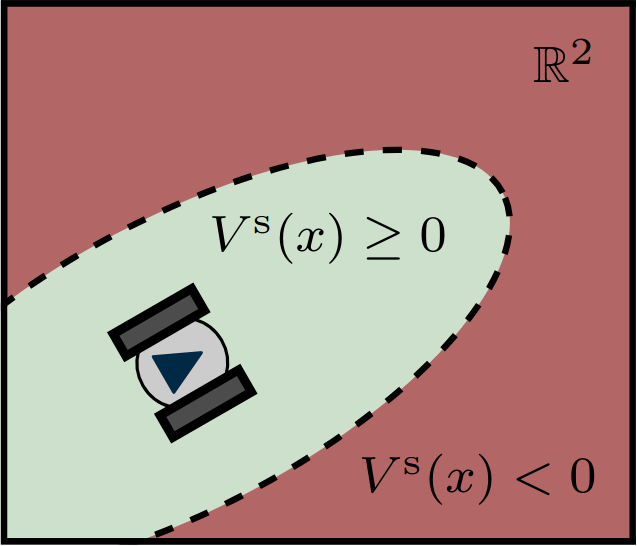
\includegraphics[width=0.25\linewidth]{./img/safety_control.png}
        \end{figure}

        \begin{remark}
            The time derivative of $V^s(\x(t))$ along the system trajectories is given by:
            \[
                \begin{split}
                    \frac{d}{dt} V^s(\x(t)) 
                    &= \nabla V^s(\x(t))^T \frac{d}{dt} \x(t) \\
                    &= \nabla V^s(\x(t))^T \Big( f(\x(t)) + g(\x(t)) \u(t) \Big) \\
                    &= \nabla V^s(\x(t))^T f(\x(t)) + \sum_{h=1}^{m} \Big( \nabla V^s(\x(t))^T g_h(\x(t)) \u_h(t) \Big)\\
                    &= L_f V^s(\x(t)) + L_g V^s(\x(t)) \u(t) \\
                \end{split}
            \]
            where $L_h V^s(\x(t)) = \nabla V^s(\x(t))^T h(\x(t))$ is the lie derivative.
        \end{remark}

    \item[Control barrier function (CBF)] \marginnote{Control barrier function (CBF)}
        A function $V^s$ is a control barrier function if there exists a continuous strictly increasing function $\gamma: \mathbb{R} \rightarrow \mathbb{R}$ with $\gamma(0) = 0$ such that the following inequality (control barrier certificate) holds:
        \[
            \sup_{\u \in U} \{ L_fV^s(\x) + L_gV^s(\x)\u + \gamma(V^s(\x)) \} \geq 0 \quad \forall \x \in X
        \]
        $\gamma$ can be interpreted as a degree of movement freedom since, as long as it holds that $V^s(\x(t)) > 0$, it is allowed that $\frac{d}{dt} V^s(\x(t)) < 0$ (i.e., the agent can move closer to the border between safe and unsafe region).

        \begin{remark}
            In principle, the negative part of $\gamma$ is not necessary (the agent should start in a safe area). However, as it is strictly increasing, it allows to move out the unsafe region if the agent ever ends up there.
        \end{remark}

        \begin{example}
            A simple choice for $\gamma$ is a linear function $\gamma(r) = \gamma r$ with $\gamma > 0$.
        \end{example}

    \item[Set of admissible safe controllers] \marginnote{Set of admissible safe controllers}
        The set of inputs that satisfy the control barrier certificate for a given state $\x$ is:
        \[
            U^s(\x) = \{ \u \in U \mid L_f V^s(\x) + L_g V^s(\x) \u + \gamma(V^s(\x)) \geq 0 \}
        \]
\end{description}


\section{Safety filter via control barrier certificate}

\begin{description}
    \item[Safety filter via control barrier certificate] \marginnote{Safety filter via control barrier certificate}
        Given a possibly unsafe reference input (from the high-level controller) $\u^\text{ref}(\x) \in \mathbb{R}^m$, the safety controller (i.e., rectifying controller) based on the control barrier certificate is designed to be minimally invasive (i.e., alter the reference as little as possible). 
        
        The policy $\u = \kappa^s(\x)$ can be defined as:
        \[
            \begin{gathered}
                \kappa^s(\x) = \arg\min_{\u \in U} \Vert \u - \u^\text{ref}(\x) \Vert^2 \\
                \text{subject to } -L_fV^s(\x) - L_gV^s(\x)\u - \gamma(V^s(\x)) \leq 0
            \end{gathered}
        \]

        \begin{remark}
            In the general case, this problem should be solved at each $t \geq 0$.
        \end{remark}


    \item[Single integrator model] \marginnote{Single integrator model}
        Control-affine non-linear dynamical system where $f(\x(t)) = 0$ and $g(\x(t)) = \matr{I}$. The dynamics is:
        \[
            \begin{split}
                \dot{\x} 
                &= 0 + \matr{I}\u \\ 
                &= \u
            \end{split}
        \]
        with $\x \in \mathbb{R}^d$ and $\u \in \mathbb{R}^d$.

        \begin{remark}
            In the case of single integrators, we have that:
           \begin{itemize}
            \item $L_f V^s(\x) = \nabla V^s(\x)^T 0 = 0$,
            \item $L_g V^s(\x) = \nabla V^s(\x)^T \matr{I} = \nabla V^s(\x)^T$.
           \end{itemize}
           Therefore:
           \[
                \begin{split}
                    \frac{d}{dt} V^s(\x(t)) 
                    &= L_f V^s(\x(t)) + L_g V^s(\x(t)) \u(t) \\
                    &= \nabla V^s(\x(t))^T \u(t)
                \end{split}
           \]
        \end{remark}
\end{description}


\subsection{Single-robot obstacle avoidance with single integrator models}

\begin{description}
    \item[Single-robot obstacle avoidance] \marginnote{Single-robot obstacle avoidance} 
        Task where the goal is to keep an agent to a safety distance $\Delta > 0$ from an obstacle.

        \begin{figure}[H]
            \centering
            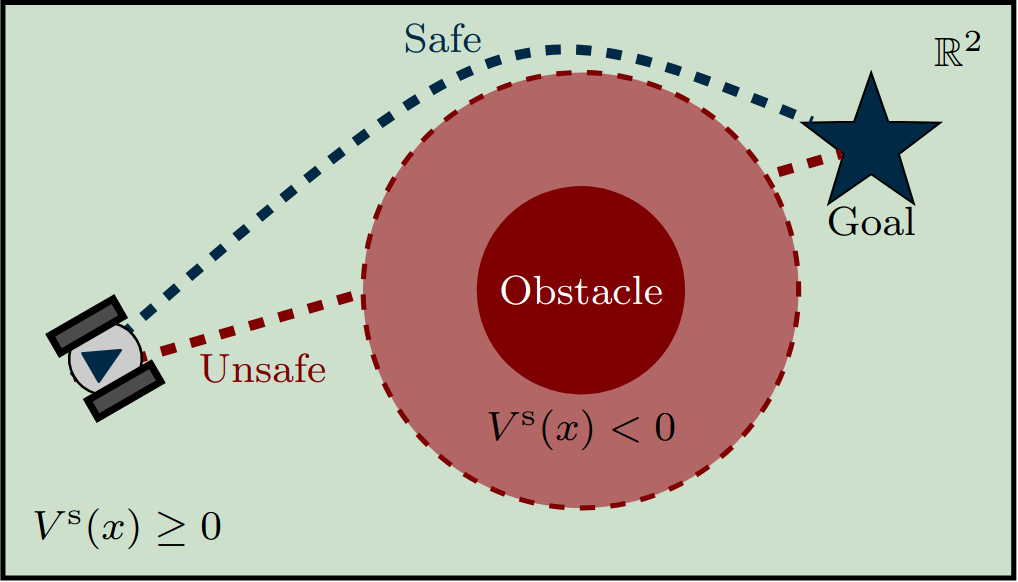
\includegraphics[width=0.35\linewidth]{./img/safety_control_single.png}
        \end{figure}

        A control barrier function to solve the task can be:
        \[
            V^s(\x) = \Vert \x - \x_\text{obs} \Vert^2 - \Delta^2
            \qquad
            \nabla V^s(\x) = 2(\x - \x_\text{obs})
        \]

        The CBF-based safety policy $\kappa^s(\x)$ can be obtained by solving:
        \[
            \begin{gathered}
                \arg\min_{\u \in U} \Vert \u - \u^\text{ref}(\x) \Vert^2 \\
                \text{subject to } -2(\x-\x_\text{obs})^T \u - \gamma(\Vert \x-\x_\text{obs} \Vert^2 - \Delta^2) \leq 0
            \end{gathered}
        \]

        As there are two constants in the constraint $a = -2(\x-\x_\text{obs})^T$ and $b = \gamma(\Vert \x-\x_\text{obs} \Vert^2 - \Delta^2)$, the problem can be reformulated as:
        % \[
        %     \arg\min_{\u \in U} \u^T\u - 2\u^T\u^\text{ref} \quad \text{subject to } a^T \u + b \leq 0
        % \]
        \[
            \arg\min_{\u \in U} \Vert \u - \u^\text{ref}(\x) \Vert^2 \quad \text{subject to } a^T \u + b \leq 0
        \]
        
        \begin{remark}
            If $U$ is a polytope (or unconstrained: $U = \mathbb{R}^d$), the problem becomes a quadratic program.
        \end{remark}
\end{description}


\subsection{Multi-robot collision avoidance with single integrator models}


\begin{description}
    \item[Multi-robot collision avoidance] \marginnote{Multi-robot collision avoidance}
        Task with $N$ single integrator agents that want to keep a safety distance $\Delta > 0$ among them.

        \begin{figure}[H]
            \centering
            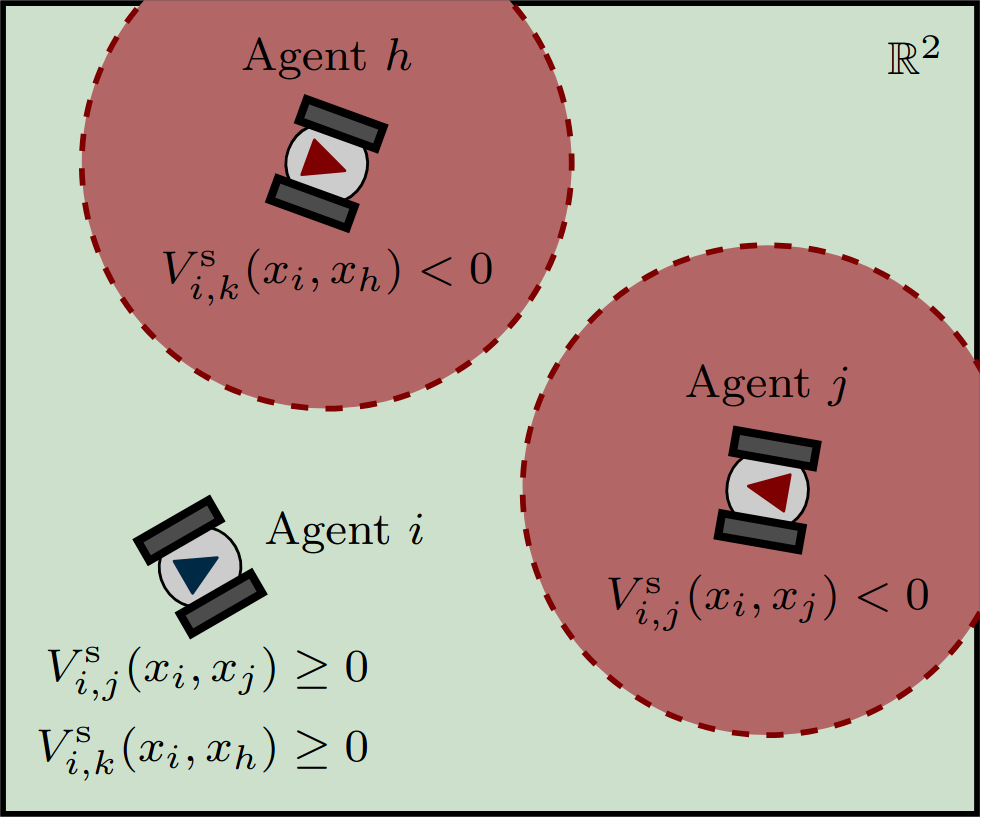
\includegraphics[width=0.35\linewidth]{./img/safety_control_multi.png}
        \end{figure}

        The local control barrier function to solve the task can be defined as:
        \[
            V^s_{i,j}(\x_i, \x_j) = \Vert \x_i - \x_j \Vert^2 - \Delta^2
            \qquad
            \begin{aligned}
                \nabla_{[\x_i]} V_{i,j}^s(\x_i, \x_j) &= 2(\x_i - \x_j) \\
                \nabla_{[\x_j]} V_{i,j}^s(\x_i, \x_j) &= 2(\x_j - \x_i)
            \end{aligned}
        \]
        The safe region $X_i$ for agent $i$ can be defined as:
        \[
            X_i = \{ \x \in \mathbb{R}^d \mid \forall j \in \mathcal{N}_i: V_{i,j}^s(\x) \geq 0 \}
        \]
\end{description}